\documentclass[14pt]{extbook}
\usepackage{multicol, enumerate, enumitem, hyperref, color, soul, setspace, parskip, fancyhdr} %General Packages
\usepackage{amssymb, amsthm, amsmath, latexsym, units, mathtools} %Math Packages
\everymath{\displaystyle} %All math in Display Style
% Packages with additional options
\usepackage[headsep=0.5cm,headheight=12pt, left=1 in,right= 1 in,top= 1 in,bottom= 1 in]{geometry}
\usepackage[usenames,dvipsnames]{xcolor}
\usepackage{dashrule}  % Package to use the command below to create lines between items
\newcommand{\litem}[1]{\item#1\hspace*{-1cm}\rule{\textwidth}{0.4pt}}
\pagestyle{fancy}
\lhead{Progress Quiz 7}
\chead{}
\rhead{Version B}
\lfoot{3510-5252}
\cfoot{}
\rfoot{Summer C 2021}
\begin{document}

\begin{enumerate}
\litem{
Write the equation of the graph presented below in the form $f(x)=ax^2+bx+c$, assuming  $a=1$ or $a=-1$. Then, choose the intervals that $a, b,$ and $c$ belong to.
\begin{center}
    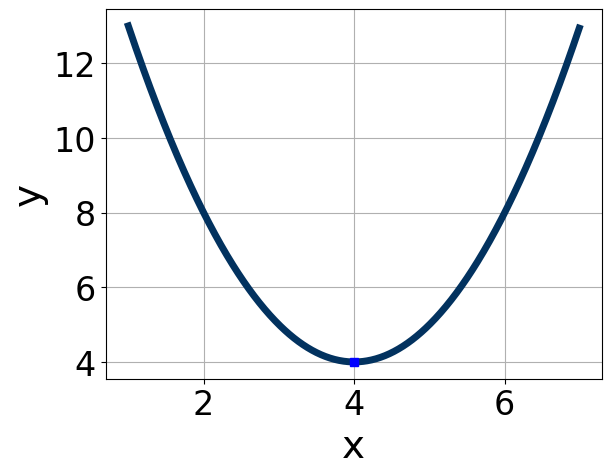
\includegraphics[width=0.5\textwidth]{../Figures/quadraticGraphToEquationB.png}
\end{center}
\begin{enumerate}[label=\Alph*.]
\item \( a \in [-2.5, -0.1], \hspace*{5mm} b \in [5, 10], \text{ and } \hspace*{5mm} c \in [-13, -8] \)
\item \( a \in [-2.5, -0.1], \hspace*{5mm} b \in [-11, -6], \text{ and } \hspace*{5mm} c \in [-13, -8] \)
\item \( a \in [-0.4, 2.4], \hspace*{5mm} b \in [-11, -6], \text{ and } \hspace*{5mm} c \in [20, 22] \)
\item \( a \in [-0.4, 2.4], \hspace*{5mm} b \in [5, 10], \text{ and } \hspace*{5mm} c \in [20, 22] \)
\item \( a \in [-0.4, 2.4], \hspace*{5mm} b \in [5, 10], \text{ and } \hspace*{5mm} c \in [11, 17] \)

\end{enumerate} }
\litem{
Solve the quadratic equation below. Then, choose the intervals that the solutions $x_1$ and $x_2$ belong to, with $x_1 \leq x_2$.\[ 25x^{2} +10 x -24 = 0 \]\begin{enumerate}[label=\Alph*.]
\item \( x_1 \in [-1.72, -0.86] \text{ and } x_2 \in [0.63, 1.34] \)
\item \( x_1 \in [-2.91, -2.08] \text{ and } x_2 \in [0.24, 0.61] \)
\item \( x_1 \in [-6.27, -5.37] \text{ and } x_2 \in [0.07, 0.26] \)
\item \( x_1 \in [-30.9, -29.8] \text{ and } x_2 \in [19.64, 20.07] \)
\item \( x_1 \in [-0.71, -0.21] \text{ and } x_2 \in [1.44, 2.11] \)

\end{enumerate} }
\litem{
Factor the quadratic below. Then, choose the intervals that contain the constants in the form $(ax+b)(cx+d); b \leq d.$\[ 16x^{2} -8 x -15 \]\begin{enumerate}[label=\Alph*.]
\item \( a \in [3.09, 4.32], \hspace*{5mm} b \in [-7, 2], \hspace*{5mm} c \in [3.36, 4.31], \text{ and } \hspace*{5mm} d \in [-3, 8] \)
\item \( a \in [7.27, 8.73], \hspace*{5mm} b \in [-7, 2], \hspace*{5mm} c \in [1.7, 2.33], \text{ and } \hspace*{5mm} d \in [-3, 8] \)
\item \( a \in [0.89, 1.59], \hspace*{5mm} b \in [-26, -15], \hspace*{5mm} c \in [0.43, 1.16], \text{ and } \hspace*{5mm} d \in [10, 15] \)
\item \( a \in [1.85, 2.78], \hspace*{5mm} b \in [-7, 2], \hspace*{5mm} c \in [7.25, 8.92], \text{ and } \hspace*{5mm} d \in [-3, 8] \)
\item \( \text{None of the above.} \)

\end{enumerate} }
\litem{
Write the equation of the graph presented below in the form $f(x)=ax^2+bx+c$, assuming  $a=1$ or $a=-1$. Then, choose the intervals that $a, b,$ and $c$ belong to.
\begin{center}
    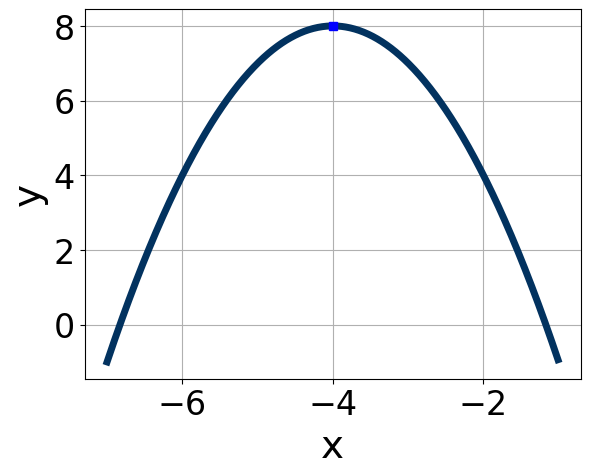
\includegraphics[width=0.5\textwidth]{../Figures/quadraticGraphToEquationCopyB.png}
\end{center}
\begin{enumerate}[label=\Alph*.]
\item \( a \in [-3, 0], \hspace*{5mm} b \in [8, 12], \text{ and } \hspace*{5mm} c \in [-9, -4] \)
\item \( a \in [-3, 0], \hspace*{5mm} b \in [-11, -6], \text{ and } \hspace*{5mm} c \in [-9, -4] \)
\item \( a \in [-3, 0], \hspace*{5mm} b \in [8, 12], \text{ and } \hspace*{5mm} c \in [-26, -22] \)
\item \( a \in [1, 4], \hspace*{5mm} b \in [-11, -6], \text{ and } \hspace*{5mm} c \in [22, 27] \)
\item \( a \in [1, 4], \hspace*{5mm} b \in [8, 12], \text{ and } \hspace*{5mm} c \in [22, 27] \)

\end{enumerate} }
\litem{
Graph the equation below.\[ f(x) = (x-2)^2 + 11 \]\begin{enumerate}[label=\Alph*.]
\begin{multicols}{2}\item 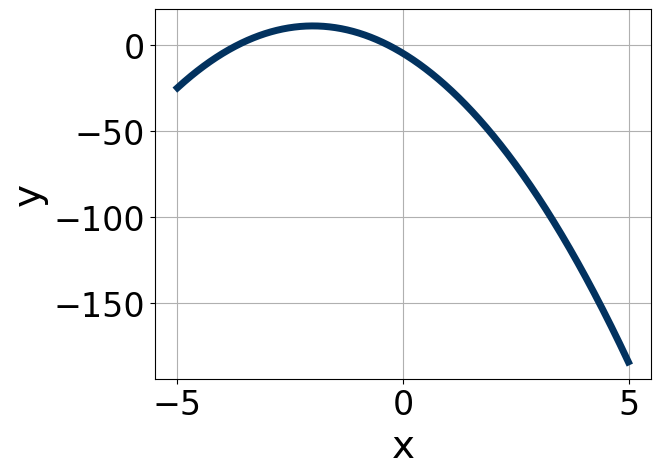
\includegraphics[width = 0.3\textwidth]{../Figures/quadraticEquationToGraphAB.png}\item 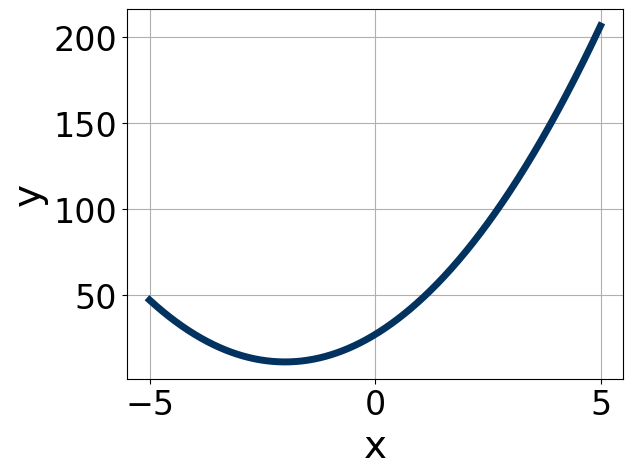
\includegraphics[width = 0.3\textwidth]{../Figures/quadraticEquationToGraphBB.png}\item 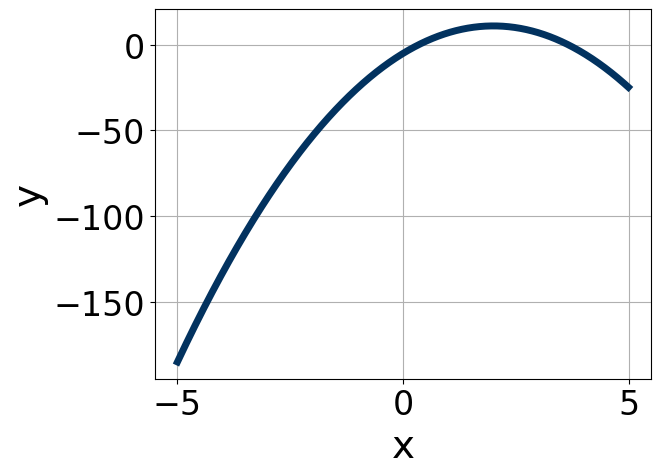
\includegraphics[width = 0.3\textwidth]{../Figures/quadraticEquationToGraphCB.png}\item 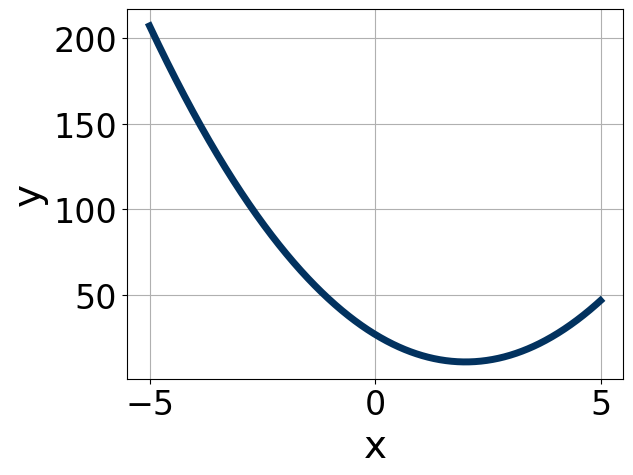
\includegraphics[width = 0.3\textwidth]{../Figures/quadraticEquationToGraphDB.png}\end{multicols}\item None of the above.
\end{enumerate} }
\litem{
Solve the quadratic equation below. Then, choose the intervals that the solutions belong to, with $x_1 \leq x_2$ (if they exist).\[ -10x^{2} -15 x + 2 = 0 \]\begin{enumerate}[label=\Alph*.]
\item \( x_1 \in [-19.3, -16.5] \text{ and } x_2 \in [16.6, 17.1] \)
\item \( x_1 \in [-0.5, 1.1] \text{ and } x_2 \in [1.3, 2.2] \)
\item \( x_1 \in [-3.6, -1.4] \text{ and } x_2 \in [-0.6, 0.6] \)
\item \( x_1 \in [-1.6, -0.9] \text{ and } x_2 \in [16.2, 16.5] \)
\item \( \text{There are no Real solutions.} \)

\end{enumerate} }
\litem{
Solve the quadratic equation below. Then, choose the intervals that the solutions $x_1$ and $x_2$ belong to, with $x_1 \leq x_2$.\[ 25x^{2} +60 x + 36 = 0 \]\begin{enumerate}[label=\Alph*.]
\item \( x_1 \in [-3.4, -1.82] \text{ and } x_2 \in [-0.68, -0.56] \)
\item \( x_1 \in [-4.42, -3.57] \text{ and } x_2 \in [-0.58, -0.25] \)
\item \( x_1 \in [-1.43, -0.68] \text{ and } x_2 \in [-1.26, -1.18] \)
\item \( x_1 \in [-6.71, -4.51] \text{ and } x_2 \in [-0.35, -0.02] \)
\item \( x_1 \in [-30.83, -29.51] \text{ and } x_2 \in [-30.04, -29.95] \)

\end{enumerate} }
\litem{
Graph the equation below.\[ f(x) = -(x-3)^2 - 18 \]\begin{enumerate}[label=\Alph*.]
\begin{multicols}{2}\item 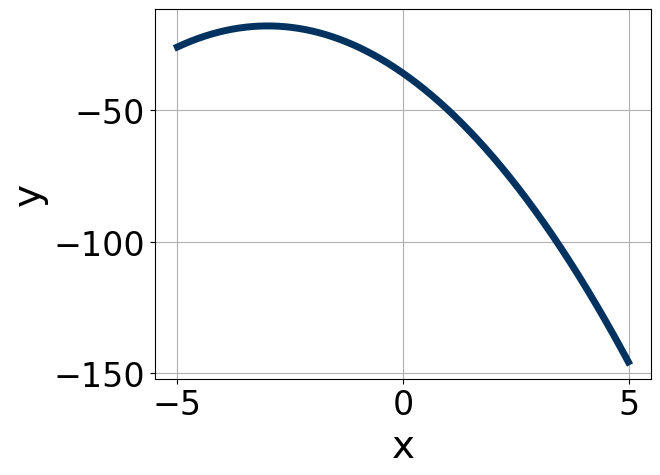
\includegraphics[width = 0.3\textwidth]{../Figures/quadraticEquationToGraphCopyAB.png}\item 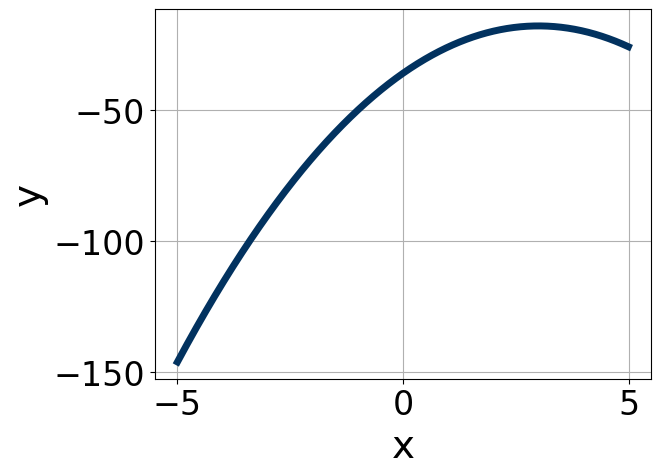
\includegraphics[width = 0.3\textwidth]{../Figures/quadraticEquationToGraphCopyBB.png}\item 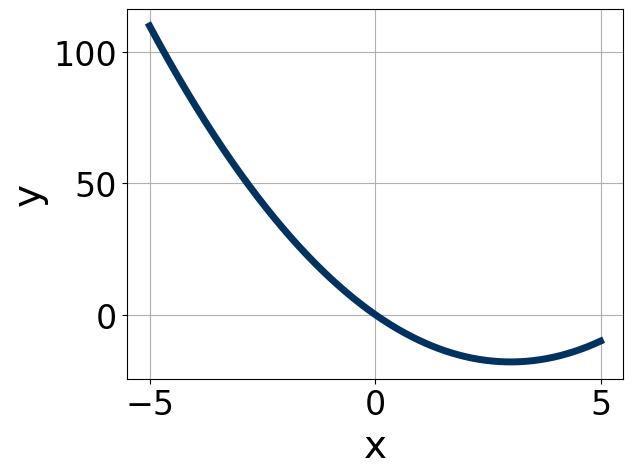
\includegraphics[width = 0.3\textwidth]{../Figures/quadraticEquationToGraphCopyCB.png}\item 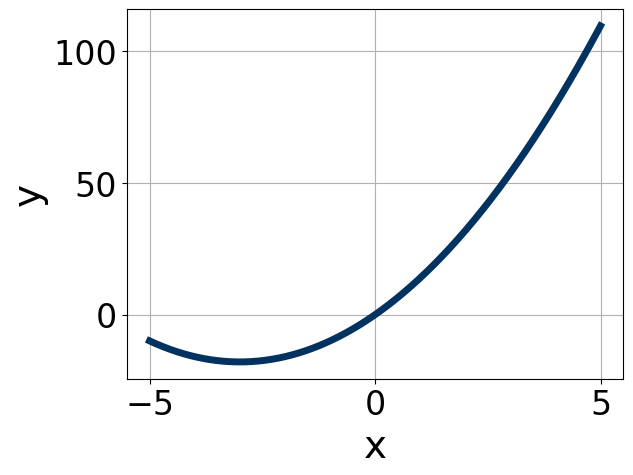
\includegraphics[width = 0.3\textwidth]{../Figures/quadraticEquationToGraphCopyDB.png}\end{multicols}\item None of the above.
\end{enumerate} }
\litem{
Solve the quadratic equation below. Then, choose the intervals that the solutions belong to, with $x_1 \leq x_2$ (if they exist).\[ 18x^{2} -14 x -6 = 0 \]\begin{enumerate}[label=\Alph*.]
\item \( x_1 \in [-25.9, -23.6] \text{ and } x_2 \in [24.99, 25.75] \)
\item \( x_1 \in [-6.8, -4.8] \text{ and } x_2 \in [18.51, 19.73] \)
\item \( x_1 \in [-2.6, -0.4] \text{ and } x_2 \in [-0.51, 0.31] \)
\item \( x_1 \in [-0.6, -0.2] \text{ and } x_2 \in [0.98, 1.55] \)
\item \( \text{There are no Real solutions.} \)

\end{enumerate} }
\litem{
Factor the quadratic below. Then, choose the intervals that contain the constants in the form $(ax+b)(cx+d); b \leq d.$\[ 36x^{2} +7 x -15 \]\begin{enumerate}[label=\Alph*.]
\item \( a \in [1.2, 4.7], \hspace*{5mm} b \in [-11, 5], \hspace*{5mm} c \in [6.3, 8.6], \text{ and } \hspace*{5mm} d \in [2, 5] \)
\item \( a \in [6.8, 9.5], \hspace*{5mm} b \in [-11, 5], \hspace*{5mm} c \in [1.8, 4.8], \text{ and } \hspace*{5mm} d \in [2, 5] \)
\item \( a \in [26.6, 27.8], \hspace*{5mm} b \in [-11, 5], \hspace*{5mm} c \in [-0.9, 1.5], \text{ and } \hspace*{5mm} d \in [2, 5] \)
\item \( a \in [-0.1, 2.7], \hspace*{5mm} b \in [-24, -16], \hspace*{5mm} c \in [-0.9, 1.5], \text{ and } \hspace*{5mm} d \in [27, 30] \)
\item \( \text{None of the above.} \)

\end{enumerate} }
\end{enumerate}

\end{document}